% !TEX program = pdflatex
\documentclass[10pt,a4paper]{article}

% -----------------------
% Encoding + language
% -----------------------
\usepackage[T1]{fontenc}
\usepackage[utf8]{inputenc}
\usepackage[english]{babel}

% -----------------------
% Scalable fonts (fixes pdfTeX microtype expansion issues)
% -----------------------
\usepackage{lmodern}

% -----------------------
% Typography (safe microtype config)
% -----------------------
\usepackage[final]{microtype}
% If your setup still complains, uncomment the next line:
% \microtypesetup{expansion=false}

% -----------------------
% Page layout
% -----------------------
\usepackage{geometry}
\geometry{margin=1.8cm}
\usepackage{subcaption}

\usepackage{setspace}
\onehalfspacing

% -----------------------
% Math + symbols
% -----------------------
\usepackage{amsmath,amssymb}

% -----------------------
% Figures + tables
% -----------------------
\usepackage{graphicx}
\usepackage{float}
\usepackage{booktabs}

% -----------------------
% Links
% -----------------------
\usepackage[hidelinks]{hyperref}

% -----------------------
% Code listings (optional)
% -----------------------
\usepackage{xcolor}
\usepackage{listings}
\lstset{
  basicstyle=\ttfamily\small,
  breaklines=true,
  frame=single,
  columns=fullflexible,
  showstringspaces=false
}

% -----------------------
% Nice lists
% -----------------------
\usepackage{enumitem}
\setlist{noitemsep, topsep=0.3em}

% -----------------------
% Pipeline Visualisation
% -----------------------
\usepackage{tikz}
\usetikzlibrary{arrows.meta, positioning}

% -----------------------
% Title meta
% -----------------------
\title{Radar Visualization Pipeline Report}
\author{Aiysha Mei Frutiger, Sandro Barbazza, Senanur Ates,  \\ University of Basel \\ Computer Architecture}
\date{January 19, 2026}

\begin{document}
\maketitle

\begin{abstract}
% TODO(Abstract): -> Sandro
%Replace with 150--250 words that state goal + concrete results (e.g., "We successfully ...").
We built a simple ultrasonic ``radar-style'' scanner that measures distance and visualizes the results live in 2D. An Arduino triggers a URM37 ultrasonic sensor, measures the echo pulse width, converts it to centimeters, and sends one newline-terminated record per sample in the format \texttt{angle,cm}. A servo sweeps the sensor so that each reading becomes an \textit{(angle, distance)} pair that can be drawn in polar coordinates on the host.

The system works reliably for typical indoor test objects: stationary targets produce consistent detections across multiple sweeps, and missing or out-of-range echoes are sent as \texttt{-1} and do not create false points in the visualization. The angular resolution is determined by the sweep step size (2$^\circ$), and the host visualization maintains a bounded state by storing only the latest measurement per angle bucket. Overall, the project demonstrates an end-to-end pipeline from ultrasonic time-of-flight measurement on an Arduino to a real-time radar-style visualization on a computer.
\end{abstract}

\vspace{-2.2em}
\begingroup
\renewcommand{\contentsname}{}%
\tableofcontents
\endgroup

\newpage

% ==========================================================
\section{Introduction}

The system is assembled from off-the-shelf components (Arduino Uno, URM37, SG90) and communicates via a newline-framed USB-serial stream (\texttt{angle,cm}) to a host-side Processing visualization. The goal is to make the full hardware--software stack observable, from echo timing on the microcontroller to real-time rendering on the PC.

\paragraph{Contributions.}
\begin{itemize}
  \item End-to-end ultrasonic scan pipeline from time-of-flight echo to live 2D visualization.
  \item Arduino firmware for servo sweep, echo-to-distance conversion, and a newline-framed serial protocol.
  \item Processing-based visualization with robust line parsing and bucket-based refresh behavior.
\end{itemize}

% ==========================================================
\section{Methodology}

\subsection{System-level approach}
% TODO(Methodology/System-level): -> Aiysha
%1--2 sentences on *method choices/assumptions* (not implementation details),
% e.g., why ASCII newline framing was chosen (debuggability/simplicity), and what the target behaviour is.
We use a simple text-based protocol (\texttt{angle,cm} per line) to keep debugging and integration straightforward across hardware and software. Newline framing defines clear message boundaries on top of the raw serial byte stream.

\paragraph{Pipeline.}
\begin{center}
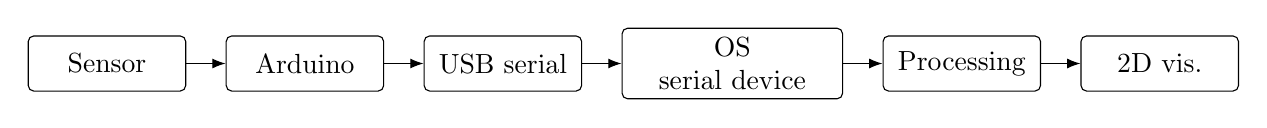
\begin{tikzpicture}[
  box/.style={draw, rounded corners=2pt, minimum height=7mm, minimum width=20mm, align=center},
  arr/.style={-Latex}
]
\node[box] (s) {Sensor};
\node[box, right=5mm of s] (a) {Arduino};
\node[box, right=5mm of a] (u) {USB serial};
\node[box, right=5mm of u, minimum width=28mm] (os) {OS\\serial device};
\node[box, right=5mm of os] (p) {Processing};
\node[box, right=5mm of p] (v) {2D vis.};

\draw[arr] (s) -- (a);
\draw[arr] (a) -- (u);
\draw[arr] (u) -- (os);
\draw[arr] (os) -- (p);
\draw[arr] (p) -- (v);
\end{tikzpicture}
\end{center}

\subsection{Implementation path}
% TODO(Methodology/Implementation path): -> Aiysha/Sena ?
% Optionally add 1 sentence about what exactly was unstable
% (e.g., framing/partial reads/reset timing), and what Processing improved (event-driven reads, line framing).
We first prototyped the UI in C using \texttt{raylib}, but the end-to-end system was unstable on Windows due to low-level serial I/O issues (port selection, reset timing, partial lines, contention). We therefore switched to Processing to simplify serial handling using its line-based, event-driven serial library and to iterate faster.


\subsection{Constraints and iterations}
% TODO(Methodology/Constraints): -> Sandro
% Add 2--4 sentences if relevant:
% - servo unavailable early -> simulated sweep mode
% - any goal changes (range, FOV, etc.)
During early development, the hardware prototype did not yet provide a reliable real angle because the servo was not available. To still build and test the full visualization pipeline, we implemented a simulated sweep angle on the host side that increments from $0^\circ$ to $180^\circ$ and back. Once the Arduino started sending \texttt{angle,cm} records, the Processing sketch automatically switched from simulated angles to real angles from the serial stream.

On the mechanical side, the delivered servo bracket did not fit our intended mounting. We therefore built a custom bracket to mount the URM37 securely and maintain a stable sweep plane.


% ==========================================================
\section{Implementation}

\subsection{Hardware}
% TODO(Implementation/Hardware): -> Sandro
% Add reproducible setup details:
% - components used (Arduino model, ultrasonic sensor model, servo model)
% - wiring summary (pins for trig/echo, servo PWM pin, power)
% - mechanical mount/stand notes (if essential)
% Keep it short but precise.
\paragraph{Bill of materials.}
Arduino Uno Rev3, URM37 ultrasonic sensor, SG90 micro servo, breadboard and jumper wires, external 5\,V / 2\,A supply, and decoupling capacitors (470\,$\mu$F, 100\,nF). The total hardware cost was approximately CHF 98.50 (excluding shipping).

\paragraph{Power and decoupling.}
The Arduino is connected to the host via USB for programming and serial communication. The SG90 servo is powered from the external 5\,V / 2\,A supply to avoid brownouts on the Arduino's 5\,V rail during movement. All grounds (Arduino, sensor, and external supply) are connected to a common ground.

For decoupling, we placed the 470\,$\mu$F electrolytic capacitor directly across the servo supply pins (5\,V to GND) close to the servo connector to buffer short current spikes during movement. In addition, a 100\,nF ceramic capacitor is placed across the URM37 supply pins close to the sensor to filter high-frequency noise on the sensor's power rail.

\paragraph{Pin connections.}
\begin{itemize}
  \item URM37 \texttt{ECHO} (Pin 4) $\rightarrow$ Arduino \texttt{D3} (\texttt{URECHO})
  \item URM37 \texttt{COMP/TRIG} (Pin 6) $\rightarrow$ Arduino \texttt{D5} (\texttt{URTRIG})
  \item SG90 servo signal $\rightarrow$ Arduino \texttt{D9} (\texttt{SERVO\_PIN})
  \item URM37 \texttt{VCC} $\rightarrow$ Arduino \texttt{5V}, \quad URM37 \texttt{GND} $\rightarrow$ Arduino \texttt{GND}
  \item SG90 servo \texttt{VCC} $\rightarrow$ external \texttt{5V}, \quad SG90 servo \texttt{GND} $\rightarrow$ common \texttt{GND}
\end{itemize}

\medskip
\noindent The URM37 sensor is mounted on a self-made servo bracket such that the sweep plane remains stable during scanning.

\subsection{Servo sweep control}
% TODO(Implementation/Servo): -> Sena
% Add concrete parameters and behaviour:
% - angle range (e.g., 15--165), step size (deg), delay between steps
% - PWM library (Servo.h) and how angle is updated
% - how sweep direction changes at boundaries
% (write here)

Sweeping is implemented with \texttt{Servo.h}. The servo moves from \texttt{MIN\_ANGLE} to \texttt{MAX\_ANGLE} in
steps of \texttt{STEP\_ANGLE} and then reverses back.

\paragraph{Parameters.}
\texttt{MIN\_ANGLE=0}, \texttt{MAX\_ANGLE=180}, \texttt{STEP\_ANGLE=2}, \texttt{SERVO\_SETTLE\_MS=30 ms},
\texttt{BETWEEN\_READ\_MS=10 ms}. A settling delay is used before each measurement to reduce motion-related errors.


\subsection{Measurement and serial protocol}
% TODO(Implementation/Measurement): -> Aiysha/Sena ?
% Add missing *exact* conversion and edge cases:
% - formula from echo duration to cm (e.g., t/58 or t/50 depending on sensor mode)
% - timeouts / invalid detection criteria -> when you send -1

% TODO(Implementation/Protocol):  -> Aiysha/Sena ?
% Add missing protocol constants:
% - baud rate (e.g., 9600)
% - exact record format: "angle,cm\n" and value ranges
The ultrasonic sensor returns an \emph{echo pulse width} proportional to time-of-flight. The Arduino triggers the sensor, measures the echo duration (e.g., with \texttt{pulseIn}), converts it to a distance in centimeters, and sends one newline-terminated ASCII record per measurement \texttt{angle,cm}.

Distance is derived from the URM37 echo pulse width $t$ (in $\mu$s) using:
\[
\text{cm} = \frac{t}{50}.
\]
If \texttt{pulseIn} times out or the measured pulse width exceeds a threshold (e.g., $t \ge 50000\,\mu\text{s}$), the firmware outputs \texttt{-1}.
Serial runs at \texttt{9600} baud and sends one record per sample as \verb|angle,cm\n|.


\subsection{Host-side data flow}
% TODO(Implementation/Host): -> Aiysha/Sena ?
% Add missing operational details:
% - how the serial port is selected/opened (manual name or auto-detect)
% - how you handle startup garbage/Arduino reset (discard first N lines, wait for "Init", etc.)
Over USB this data is exposed by the OS as a serial device, which Processing reads as a byte stream, frames into lines, parses angle and distance, and uses to update the visualization state.
On Arduino boards, opening the serial port can reset the microcontroller; therefore the Processing sketch ignores initial startup lines until valid \texttt{angle,cm} records are received.

\paragraph{Pipeline.}
\begin{center}
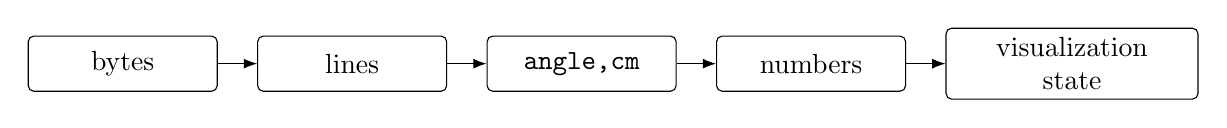
\begin{tikzpicture}[
  box/.style={draw, rounded corners=2pt, minimum height=7mm, minimum width=24mm, align=center},
  arr/.style={-Latex}
]
\node[box] (b) {bytes};
\node[box, right=5mm of b] (l) {lines};
\node[box, right=5mm of l] (t) {\texttt{angle,cm}};
\node[box, right=5mm of t] (n) {numbers};
\node[box, right=5mm of n, minimum width=32mm] (st) {visualization\\state};

\draw[arr] (b) -- (l);
\draw[arr] (l) -- (t);
\draw[arr] (t) -- (n);
\draw[arr] (n) -- (st);
\end{tikzpicture}
\end{center}

\subsection{Visualization}
% TODO(Implementation/Visualization): -> Aiysha/Sena ?
% Ensure consistency:
% - In Introduction you mention polar coordinates; here you use 15--165 deg FOV. Make sure this matches servo sweep.

The visualization renders a radar-style scan over a $0^\circ$--$180^\circ$ field of view. A sweep line indicates the current angle, and each incoming $(\textit{angle}, \textit{distance})$ measurement is mapped to polar coordinates to draw a point at the corresponding radius. A static grid (concentric arcs and radial lines) provides scale and orientation.

\subsection{Serial parsing and ``bucket'' state}
% TODO(Implementation/Parsing): -> Aiysha/Sena ?
% Add missing failure handling details:
% - what happens on malformed lines (ignore, log)
% - numeric parsing errors

% TODO(Implementation/Buckets): -> Aiysha/Sena ?
% Add missing parameters:
% - define ANGLE_BUCKET_DEG value
% - how many buckets -> array size and index computation
Processing receives a continuous byte stream and frames it into newline-terminated records. Each line is trimmed, split by comma, and parsed into numeric \textit{angle} and \textit{distance} values; invalid readings are encoded as \texttt{-1} (no detection).

To keep memory bounded and emulate radar refresh behavior, the scan is discretized into fixed-width angle buckets (e.g., \texttt{ANGLE\_BUCKET\_DEG}). Each bucket stores the most recent distance for its slice and is overwritten on the next sweep; a \texttt{-1} clears the corresponding bucket.

Malformed lines (wrong token count or non-numeric values) are ignored. A typical setting is \texttt{ANGLE\_BUCKET\_DEG=2} to match the servo
step size; each bucket stores the latest distance for its angle slice and is overwritten on rescan.



\subsection{Reproducibility notes}
% TODO(Implementation/Repro): -> Aiysha/Sena/Sandro
% Add 4--6 lines to let someone rerun the project:
% - required software versions (Arduino IDE, Processing version)
% - how to flash Arduino, how to start Processing sketch
% - what to configure (COM port name, baud rate)
To reproduce the project, flash the Arduino firmware using Arduino IDE 2.x and connect the board via USB. Open the Arduino Serial Monitor at \texttt{9600} baud to verify that the device outputs newline-terminated ASCII records in the form \texttt{angle,cm}, where \texttt{angle} is in $[0,180]$ and \texttt{cm} is either a non-negative distance in centimeters or \texttt{-1} for invalid/out-of-range measurements.

Then start the Processing sketch (Processing 4.x). Select the correct serial device from \texttt{Serial.list()} and open it at \texttt{9600} baud. The sketch ignores startup noise (due to Arduino reset on port open) until it receives valid \texttt{angle,cm} lines; once valid records arrive, the visualization updates continuously while the servo sweeps.

The expected behavior is a stable sweep over $0^\circ$--$180^\circ$ with detections appearing at consistent angles for stationary objects and disappearing when \texttt{-1} is received for that angle bucket.

% ==========================================================
\section{Evaluation}

\subsection{Functional validation}
% TODO(Evaluation/Functional): -> Sandro
% Report what you tested and what worked:
% - live updates, correct sweep behaviour, object detection, -1 clears, etc.
% - include 2--4 concrete observations
We validated the system incrementally. First, we verified the SG90 servo motion using fixed target angles (0$^\circ$, 90$^\circ$, 180$^\circ$). Second, we validated the URM37 distance measurement in isolation by reading the echo pulse width via \texttt{pulseIn} and converting it to centimeters. Third, we combined servo sweep and distance sensing and streamed \texttt{angle,cm} records over serial to test the end-to-end data path. Finally, we switched to explicit sensor triggering (TRIG/ECHO mode) to control measurement timing and handle missing/out-of-range echoes robustly.


\subsection{Performance and limitations}
% TODO(Evaluation/Performance): -> Sandro
% Add a few measurable or at least observable metrics:
% - max reliable distance (approx.)
% - update rate (measurements per second or sweep time)
% - angular resolution (servo step)

% TODO(Evaluation/Limitations): -> Sandro
% Briefly note known limitations (surface angle, noise, servo backlash).
The angular resolution is set by the sweep step size (\texttt{STEP\_ANGLE=2}$^\circ$), while the refresh rate depends on the servo settling time and the delay between readings (\texttt{SERVO\_SETTLE\_MS=30\,ms}, \texttt{BETWEEN\_READ\_MS=10\,ms}). Measurement stability varies with surface reflectivity and orientation; for example, a stainless-steel water bottle produced less stable readings. Very short distances were occasionally unreliable. We did not notice angle jitter from mechanical play, but we did not quantify it.



\subsection{Match with project goals}
% TODO(Evaluation/Goals): -> Sandro
% 2--3 sentences: did you meet original goal, what remains incomplete, why.
The final system meets the project goal of a compact radar-style scanner that converts ultrasonic time-of-flight into a live 2D visualization. It provides an explainable end-to-end pipeline from embedded measurement on the Arduino to host-side parsing and rendering, and it remains usable both in prototype mode (simulated sweep) and in the final mode with real servo angles. Remaining improvements would focus on calibration and filtering to further stabilize readings and on making the setup more self-contained (e.g., an integrated display and basic calibration routines).

% ==========================================================
\section{Conclusion}
We built an end-to-end ultrasonic ``radar-style'' system that converts echo time-of-flight into a live 2D visualization. The stack is observable from Arduino signal processing and USB serial transport to host-side parsing and rendering in Processing.

A key lesson was robustness across layers, especially around serial communication and integration between firmware and visualization.

\paragraph{Self-assessment and outlook.}
We kept the project intentionally simple to understand each layer of the pipeline. With more time, we would increase complexity by adding an on-device LCD (instead of a PC-based UI) and basic controls such as a power switch and calibration routine.

\paragraph{Division of labor.}
All group members assembled the hardware setup and testing. Sandro implemented the main Arduino sensing/communication code and built the stand/chassis. Senanur developed the Arduino servo sweep control. Aiysha implemented the Processing visualization, including parsing and bucket-based rendering.

% ==========================================================
\newpage
\section*{References}
\addcontentsline{toc}{section}{References}

\begin{itemize}
  \item Processing (project homepage + downloads): \url{https://processing.org/} \url{https://processing.org/download/} % :contentReference[oaicite:0]{index=0}
  \item Processing Serial library reference (Serial class): \url{https://processing.org/reference/libraries/serial/Serial.html} % :contentReference[oaicite:1]{index=1}
  \item Processing Serial library reference (bufferUntil): \url{https://processing.org/reference/libraries/serial/Serial_bufferUntil_.html} % :contentReference[oaicite:2]{index=2}
  \item Processing Serial library reference (readStringUntil — common alternative used with newline framing): \url{https://processing.org/reference/libraries/serial/Serial_readStringUntil_.html} % :contentReference[oaicite:3]{index=3}
  \item Processing Serial library reference (serialEvent): \url{https://processing.org/reference/libraries/serial/serialEvent_.html} % :contentReference[oaicite:4]{index=4}
  \item Project source code repository: \url{https://github.com/ateschsena/Radar.git}
  \item URM37 Datasheet:
  \url{http://www.farnell.com/datasheets/4376735.pdf}
\end{itemize}

%==========================================================
\section*{Declaration of Authorship}
\addcontentsline{toc}{section}{Declaration of Authorship}

ChatGPT was used solely to improve the clarity and coherence of the report's language. All ideas, analyses, 
and interpretations presented reflect the group's own work and research.

\end{document}
